
\section{Variance of Distance}\label{sec:variance}


For all the quasinorms, i.e, norms $p < 1$. The variance grows polynomially. Since the data is a sample of random datapoints, the sample variance is used.

\[
    \text{Var}(X) = \frac{1}{n -1 } \sum_{i=1}^{n} \left(X_i - \mu \right)^2
\]


\begin{equation}
    \text{Var}_{\text{sample}}\left(\|\mathbf{x}\|_p\right) = \lim_{k \to \infty} \left( \frac{1}{N - 1} \sum_{i=1}^{k} \left( \left( \sum_{i=1}^{k} |x_i|^p \right)^{\frac{1}{p}} - \mathbb{E}\left[\left( \sum_{i=1}^{k} |x_i|^p \right)^{\frac{1}{p}}\right] \right)^2 \right)
\end{equation}

Similar to the min-max-mean distance, the variance grows polynomially for all \(p < 1\). When \(p = 1\), the variance grows linearly. And when \(p \geq 2\), the variance grows proportionally to a \(\frac{1}{\log(k)}\) function.

The interesting case was the norms p between 1 and 2. For those norms, the variance goes to infinity but much slower than for the \(p=1\) linear growth.

All variances larger or equal to 2 converge to 0 as k increases. This is behavior is evident in the~\autoref{fig:avg_variance_2_5_inf}.


% \FloatBarrier  % Force the figure to appear after this point

\begin{figure}[ht!]
    \centering
    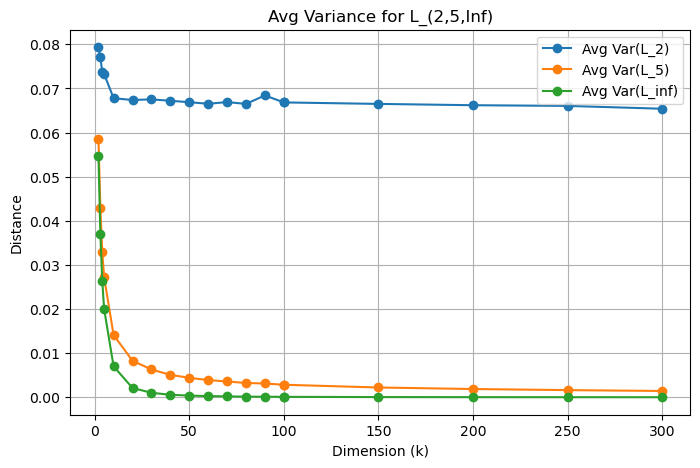
\includegraphics[width=\textwidth, height=\textheight, keepaspectratio]{avg_variance_2_5_inf.png}
    \caption{\emph{Avg Variance for \(L_{(2,5,\infty)}\)}}
    \label{fig:avg_variance_2_5_inf}
\end{figure}


% \FloatBarrier  % Force the figure to appear after this point

In summary, the curves with $p < 1$ can be characterized as polynomial curves. The curves with $ 1 < p < 2 \propto k^{1/p}$ are characterized as inverse polynomial curves.

